\chapter{Implementation Details}
\section{Case of study 1: Cluster and Honeypot for a Ransomware attack}
\section{Case of study 2: Cluster and Honeypot for a DoS attack}
\subsection{Instruments used}
In order to simulate our IoT cluster with the honeypot, we decide to implement a simulation using python. The most important aspect 
to respect when developing a client-server application, like our ioT cluster, it that the servers and the sensors have to be able to exchange data 
between each others. The module sockets present in  the python library allow us to support networking protocols between two or more processes across machines. In this particular case we use TCP sockets, where at one side a process act like a client and on the other side a process act like a server. Also python offer the module selectors that allow us to serve multiple sockets connections. In particular the .select() method allows us to check for I/O completion on more than one socket. So we can call .select() to see which sockets have I/O ready for reading and/or writing.  We also want to underline that with .select()  we’re not able to run concurrently. 
\subsection{ First structure of the IoT cluster}
In our first simulation we decided to implement an high-interaction honeypot and a cluster reported in the figure below.
\begin{figure}[h!]
  \centering
  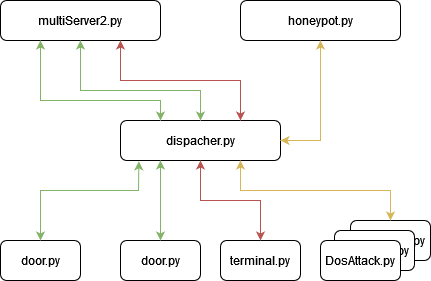
\includegraphics[width = 12cm]{images/HighInterationHoneypot.drawio.png}
  \caption{Our simple IoT cluster with an high-interaction honeypot}
  \label{fig:DosImpl1}
\end{figure}
\FloatBarrier
\noindent
We have different type of client (just like in the reality of an heterogeneous IoT cluster).
In the nexts subsections we will explain the purpose of every script and how they interact. We would like to remind that on the git repository there is also a tutorial about the use of the first version of the cluster.
\subsection{Door.py}
This script represent a door that could be controlled by our system. It have a global variable named status , that could assume 2 values, UNLOCK and LOCK.
This are the status of the door. When the "sensor" is turned on,  it send 2 packets to the server with the initial status of the door, then it wait for commands from the server.  The packets send by the door sensor have this format: "topic: DOOR data: LOCK/UNLOCK IPFALSE: 129.0.0.1". The IPFALSE filed was an attempt
to mask the loopbacks IP with external IP, but then we understand that this was not necessary. A socket can be distinguished by another by the couple (IP,port) 
of the client and the server. When the scripts from this implementation will be launch from different network, the system will behave in the same way of  our tests on loopback. We decided to leave this field because if in the future we need to exchange more data, we could recycle it, of course changhing the name.
The data that the door could receive from the server have this format: "topic: SERVER data: STATUS/LOCK/UNLOCK IPFALSE: someData". When the server 
request the status, the door check the variable STATUS and sent it value to the server.  If the command is LOCK the STATUS variable is set to LOCK, if the command is UNLOCK the STATUS variable is set to UNLOCK.


\subsection{terminal.py}
This script represent a terminal where the admin of the IoT cluster could control the sensors. The terminal offer a set of command , that are reported in the user manual.\\
As it is implemented, if the termianl do not receive a response from the server, it stops working.  In future version we could add a timer, and after some time elapsed, we stop wainting from the response and rise an error.


\subsection{dispacher.py}
The dispacher is the first line of defense controlled by our honeypot. All the new connection from outside the network are sent to the dispacher. Here we have 3 list in python, one for the trusted socket named socketWhiteList, that could communicate with the server. Every socket in the white list have a personal socket from the dispacher to the server, the couple is saved in the list coppiaSocketWhiteListSocketServer. The list socketPending save all the new connection from outside that are waiting from the response of the honeypot. When a new connection arrive to the dispacher, the packet sent are redirect to the honeypot. The packet from the dispacher to the honeypot are sent in the same socket named socket\_honey. When a response from the honeypot arrive, if the connection is approved the dispacher move the socket from the list of the pending one to the list of the whitesocket. If the connection is not approved the sockert is delete from the list of the pending one and closed forever.  When a new connection arrive, the dispache sent to the honeypot first the peer name of the new connection, and then the first packet received from it. While a connection is pending, all the other packets from outside are lost, it's just an implementation choise.

\subsection{DosAttack.py}
The script for the Dos attack is very simple,  after establish a connection it start send random data using the socket. 


\subsection{honeypot.py}
The honeypot control the packets from the new connection fro the outside to the dispacher. If the came from a terminal or a door, the new connection is approved , otherwise is not approved. The format of the data from the honeypot to the dispacher is:"ip-port: (ip, port) status: TRUSTED/UNTRUSTED" . The honeypot receive from every connection to check 2 data, the peer name that will be saved and then resent to the dispacher to specify what connection the honeypot is refeiring, and the packet to analyze. 

\subsection{multiServer2.py}
The server have to handle all the connection of the sensors. It have to connect the terminal to the doors, and send the command from the terminal to the correct door. If the command is for all the doors connected, it send a packet with the command to all of them. It have a list of sockets of the doors and a list for the socket of the terminals. As it is implemented, our system work with only one terminal connected to the server, but this could be ealisy changed. The server have to nìbe reached only by the packtes from the dispacher. 



\subsection{ Second structure of the IoT cluster}
After the presentation of our projects it was notice to our group that the honeypot and the dispacher could be collapsed in just one "server" , actualy a script, that handle all the function of the dispacher and the honeypot.  So we create the script dispacherAndPot.py . Here, we have a function named honeypot, that , like the reader probably already iìunderstand, is the honeypot. When a new connection arrive, this function is called and check the packets sent to the dispacher. If it is ok it return 1, otherwise 0. This low-interaction is much more efficient and simple, it do not lose packet from pending connection and we do not neeed to create socket between the honeypot and the dispacher. According to the complexity of the simulation right now, this implementation is much better, but if we want for example to improve the honeypot with new feature, like the ones from our other implementation, we suggest to use the first version. The picture below report the structure of the second implementation. 
\begin{figure}[h!]
  \centering
  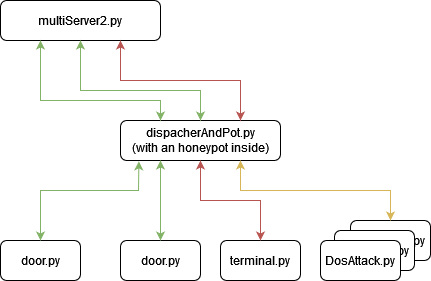
\includegraphics[width = 12cm]{images/lowInterationHoneypot.drawio.png}
  \caption{Our simple IoT cluster with a low-interaction honeypot}
  \label{fig:DosImpl2}
\end{figure}
\FloatBarrier
\noindent











%cancella
This is where you explain what you have implemented and how you have implemented it. Place here all the details that you consider important, organize the chapter in sections and subsections to explain the development and your workflow.\\Given the self-explicative title of the chapter, readers usually skip it. This is ok, because this entire chapter is simply meant to describe the details of your work so that people that are very interested (such as people who have to evaluate your work or people who have to build something more complex starting from what you did) can fully understand what you developed or implemented.\\Don't worry about placing too many details in this chapter, the only essential thing is that you keep everything tidy, without mixing too much information (so make use of sections, subsections, lists, etc.). As usual, pictures are helpful.